% Created by tikzDevice version 0.10.1 on 2016-08-15 14:57:33
% !TEX encoding = UTF-8 Unicode
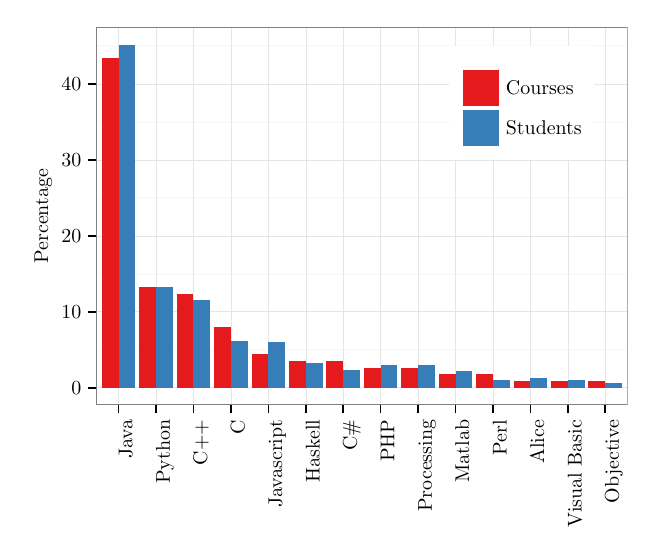
\begin{tikzpicture}[x=1pt,y=1pt]
\definecolor{fillColor}{RGB}{255,255,255}
\path[use as bounding box,fill=fillColor,fill opacity=0.00] (0,0) rectangle (216.81,180.67);
\begin{scope}
\path[clip] (  0.00,  0.00) rectangle (216.81,180.67);
\definecolor{drawColor}{RGB}{255,255,255}
\definecolor{fillColor}{RGB}{255,255,255}

\path[draw=drawColor,line width= 0.6pt,line join=round,line cap=round,fill=fillColor] (  0.00,  0.00) rectangle (216.81,180.68);
\end{scope}
\begin{scope}
\path[clip] ( 24.76, 44.37) rectangle (216.81,180.67);
\definecolor{fillColor}{RGB}{255,255,255}

\path[fill=fillColor] ( 24.76, 44.37) rectangle (216.81,180.67);
\definecolor{drawColor}{gray}{0.98}

\path[draw=drawColor,line width= 0.6pt,line join=round] ( 24.76, 64.29) --
	(216.81, 64.29);

\path[draw=drawColor,line width= 0.6pt,line join=round] ( 24.76, 91.73) --
	(216.81, 91.73);

\path[draw=drawColor,line width= 0.6pt,line join=round] ( 24.76,119.17) --
	(216.81,119.17);

\path[draw=drawColor,line width= 0.6pt,line join=round] ( 24.76,146.61) --
	(216.81,146.61);

\path[draw=drawColor,line width= 0.6pt,line join=round] ( 24.76,174.05) --
	(216.81,174.05);
\definecolor{drawColor}{gray}{0.90}

\path[draw=drawColor,line width= 0.2pt,line join=round] ( 24.76, 50.57) --
	(216.81, 50.57);

\path[draw=drawColor,line width= 0.2pt,line join=round] ( 24.76, 78.01) --
	(216.81, 78.01);

\path[draw=drawColor,line width= 0.2pt,line join=round] ( 24.76,105.45) --
	(216.81,105.45);

\path[draw=drawColor,line width= 0.2pt,line join=round] ( 24.76,132.89) --
	(216.81,132.89);

\path[draw=drawColor,line width= 0.2pt,line join=round] ( 24.76,160.33) --
	(216.81,160.33);

\path[draw=drawColor,line width= 0.2pt,line join=round] ( 32.87, 44.37) --
	( 32.87,180.67);

\path[draw=drawColor,line width= 0.2pt,line join=round] ( 46.40, 44.37) --
	( 46.40,180.67);

\path[draw=drawColor,line width= 0.2pt,line join=round] ( 59.92, 44.37) --
	( 59.92,180.67);

\path[draw=drawColor,line width= 0.2pt,line join=round] ( 73.45, 44.37) --
	( 73.45,180.67);

\path[draw=drawColor,line width= 0.2pt,line join=round] ( 86.97, 44.37) --
	( 86.97,180.67);

\path[draw=drawColor,line width= 0.2pt,line join=round] (100.50, 44.37) --
	(100.50,180.67);

\path[draw=drawColor,line width= 0.2pt,line join=round] (114.02, 44.37) --
	(114.02,180.67);

\path[draw=drawColor,line width= 0.2pt,line join=round] (127.55, 44.37) --
	(127.55,180.67);

\path[draw=drawColor,line width= 0.2pt,line join=round] (141.07, 44.37) --
	(141.07,180.67);

\path[draw=drawColor,line width= 0.2pt,line join=round] (154.60, 44.37) --
	(154.60,180.67);

\path[draw=drawColor,line width= 0.2pt,line join=round] (168.12, 44.37) --
	(168.12,180.67);

\path[draw=drawColor,line width= 0.2pt,line join=round] (181.65, 44.37) --
	(181.65,180.67);

\path[draw=drawColor,line width= 0.2pt,line join=round] (195.17, 44.37) --
	(195.17,180.67);

\path[draw=drawColor,line width= 0.2pt,line join=round] (208.70, 44.37) --
	(208.70,180.67);
\definecolor{fillColor}{RGB}{228,26,28}

\path[fill=fillColor] ( 26.79, 50.57) rectangle ( 32.87,169.56);
\definecolor{fillColor}{RGB}{55,126,184}

\path[fill=fillColor] ( 32.87, 50.57) rectangle ( 38.96,174.48);
\definecolor{fillColor}{RGB}{228,26,28}

\path[fill=fillColor] ( 40.31, 50.57) rectangle ( 46.40, 86.99);
\definecolor{fillColor}{RGB}{55,126,184}

\path[fill=fillColor] ( 46.40, 50.57) rectangle ( 52.48, 87.10);
\definecolor{fillColor}{RGB}{228,26,28}

\path[fill=fillColor] ( 53.84, 50.57) rectangle ( 59.92, 84.56);
\definecolor{fillColor}{RGB}{55,126,184}

\path[fill=fillColor] ( 59.92, 50.57) rectangle ( 66.01, 82.31);
\definecolor{fillColor}{RGB}{228,26,28}

\path[fill=fillColor] ( 67.36, 50.57) rectangle ( 73.45, 72.42);
\definecolor{fillColor}{RGB}{55,126,184}

\path[fill=fillColor] ( 73.45, 50.57) rectangle ( 79.53, 67.59);
\definecolor{fillColor}{RGB}{228,26,28}

\path[fill=fillColor] ( 80.89, 50.57) rectangle ( 86.97, 62.71);
\definecolor{fillColor}{RGB}{55,126,184}

\path[fill=fillColor] ( 86.97, 50.57) rectangle ( 93.06, 66.95);
\definecolor{fillColor}{RGB}{228,26,28}

\path[fill=fillColor] ( 94.41, 50.57) rectangle (100.50, 60.28);
\definecolor{fillColor}{RGB}{55,126,184}

\path[fill=fillColor] (100.50, 50.57) rectangle (106.58, 59.33);
\definecolor{fillColor}{RGB}{228,26,28}

\path[fill=fillColor] (107.93, 50.57) rectangle (114.02, 60.28);
\definecolor{fillColor}{RGB}{55,126,184}

\path[fill=fillColor] (114.02, 50.57) rectangle (120.11, 57.02);
\definecolor{fillColor}{RGB}{228,26,28}

\path[fill=fillColor] (121.46, 50.57) rectangle (127.55, 57.85);
\definecolor{fillColor}{RGB}{55,126,184}

\path[fill=fillColor] (127.55, 50.57) rectangle (133.63, 58.83);
\definecolor{fillColor}{RGB}{228,26,28}

\path[fill=fillColor] (134.98, 50.57) rectangle (141.07, 57.85);
\definecolor{fillColor}{RGB}{55,126,184}

\path[fill=fillColor] (141.07, 50.57) rectangle (147.16, 58.76);
\definecolor{fillColor}{RGB}{228,26,28}

\path[fill=fillColor] (148.51, 50.57) rectangle (154.60, 55.42);
\definecolor{fillColor}{RGB}{55,126,184}

\path[fill=fillColor] (154.60, 50.57) rectangle (160.68, 56.69);
\definecolor{fillColor}{RGB}{228,26,28}

\path[fill=fillColor] (162.03, 50.57) rectangle (168.12, 55.42);
\definecolor{fillColor}{RGB}{55,126,184}

\path[fill=fillColor] (168.12, 50.57) rectangle (174.21, 53.41);
\definecolor{fillColor}{RGB}{228,26,28}

\path[fill=fillColor] (175.56, 50.57) rectangle (181.65, 52.99);
\definecolor{fillColor}{RGB}{55,126,184}

\path[fill=fillColor] (181.65, 50.57) rectangle (187.73, 54.04);
\definecolor{fillColor}{RGB}{228,26,28}

\path[fill=fillColor] (189.08, 50.57) rectangle (195.17, 52.99);
\definecolor{fillColor}{RGB}{55,126,184}

\path[fill=fillColor] (195.17, 50.57) rectangle (201.26, 53.41);
\definecolor{fillColor}{RGB}{228,26,28}

\path[fill=fillColor] (202.61, 50.57) rectangle (208.70, 52.99);
\definecolor{fillColor}{RGB}{55,126,184}

\path[fill=fillColor] (208.70, 50.57) rectangle (214.78, 52.42);
\definecolor{drawColor}{gray}{0.50}

\path[draw=drawColor,line width= 0.6pt,line join=round,line cap=round] ( 24.76, 44.37) rectangle (216.81,180.67);
\end{scope}
\begin{scope}
\path[clip] (  0.00,  0.00) rectangle (216.81,180.67);
\definecolor{drawColor}{RGB}{0,0,0}

\node[text=drawColor,anchor=base east,inner sep=0pt, outer sep=0pt, scale=  0.72] at ( 19.36, 48.09) {0};

\node[text=drawColor,anchor=base east,inner sep=0pt, outer sep=0pt, scale=  0.72] at ( 19.36, 75.53) {10};

\node[text=drawColor,anchor=base east,inner sep=0pt, outer sep=0pt, scale=  0.72] at ( 19.36,102.97) {20};

\node[text=drawColor,anchor=base east,inner sep=0pt, outer sep=0pt, scale=  0.72] at ( 19.36,130.41) {30};

\node[text=drawColor,anchor=base east,inner sep=0pt, outer sep=0pt, scale=  0.72] at ( 19.36,157.85) {40};
\end{scope}
\begin{scope}
\path[clip] (  0.00,  0.00) rectangle (216.81,180.67);
\definecolor{drawColor}{RGB}{0,0,0}

\path[draw=drawColor,line width= 0.6pt,line join=round] ( 21.76, 50.57) --
	( 24.76, 50.57);

\path[draw=drawColor,line width= 0.6pt,line join=round] ( 21.76, 78.01) --
	( 24.76, 78.01);

\path[draw=drawColor,line width= 0.6pt,line join=round] ( 21.76,105.45) --
	( 24.76,105.45);

\path[draw=drawColor,line width= 0.6pt,line join=round] ( 21.76,132.89) --
	( 24.76,132.89);

\path[draw=drawColor,line width= 0.6pt,line join=round] ( 21.76,160.33) --
	( 24.76,160.33);
\end{scope}
\begin{scope}
\path[clip] (  0.00,  0.00) rectangle (216.81,180.67);
\definecolor{drawColor}{RGB}{0,0,0}

\path[draw=drawColor,line width= 0.6pt,line join=round] ( 32.87, 41.37) --
	( 32.87, 44.37);

\path[draw=drawColor,line width= 0.6pt,line join=round] ( 46.40, 41.37) --
	( 46.40, 44.37);

\path[draw=drawColor,line width= 0.6pt,line join=round] ( 59.92, 41.37) --
	( 59.92, 44.37);

\path[draw=drawColor,line width= 0.6pt,line join=round] ( 73.45, 41.37) --
	( 73.45, 44.37);

\path[draw=drawColor,line width= 0.6pt,line join=round] ( 86.97, 41.37) --
	( 86.97, 44.37);

\path[draw=drawColor,line width= 0.6pt,line join=round] (100.50, 41.37) --
	(100.50, 44.37);

\path[draw=drawColor,line width= 0.6pt,line join=round] (114.02, 41.37) --
	(114.02, 44.37);

\path[draw=drawColor,line width= 0.6pt,line join=round] (127.55, 41.37) --
	(127.55, 44.37);

\path[draw=drawColor,line width= 0.6pt,line join=round] (141.07, 41.37) --
	(141.07, 44.37);

\path[draw=drawColor,line width= 0.6pt,line join=round] (154.60, 41.37) --
	(154.60, 44.37);

\path[draw=drawColor,line width= 0.6pt,line join=round] (168.12, 41.37) --
	(168.12, 44.37);

\path[draw=drawColor,line width= 0.6pt,line join=round] (181.65, 41.37) --
	(181.65, 44.37);

\path[draw=drawColor,line width= 0.6pt,line join=round] (195.17, 41.37) --
	(195.17, 44.37);

\path[draw=drawColor,line width= 0.6pt,line join=round] (208.70, 41.37) --
	(208.70, 44.37);
\end{scope}
\begin{scope}
\path[clip] (  0.00,  0.00) rectangle (216.81,180.67);
\definecolor{drawColor}{RGB}{0,0,0}

\node[text=drawColor,rotate= 90.00,anchor=base east,inner sep=0pt, outer sep=0pt, scale=  0.72] at ( 37.83, 38.97) {Java};

\node[text=drawColor,rotate= 90.00,anchor=base east,inner sep=0pt, outer sep=0pt, scale=  0.72] at ( 51.36, 38.97) {Python};

\node[text=drawColor,rotate= 90.00,anchor=base east,inner sep=0pt, outer sep=0pt, scale=  0.72] at ( 64.88, 38.97) {C++};

\node[text=drawColor,rotate= 90.00,anchor=base east,inner sep=0pt, outer sep=0pt, scale=  0.72] at ( 78.41, 38.97) {C};

\node[text=drawColor,rotate= 90.00,anchor=base east,inner sep=0pt, outer sep=0pt, scale=  0.72] at ( 91.93, 38.97) {Javascript};

\node[text=drawColor,rotate= 90.00,anchor=base east,inner sep=0pt, outer sep=0pt, scale=  0.72] at (105.46, 38.97) {Haskell};

\node[text=drawColor,rotate= 90.00,anchor=base east,inner sep=0pt, outer sep=0pt, scale=  0.72] at (118.98, 38.97) {C\#};

\node[text=drawColor,rotate= 90.00,anchor=base east,inner sep=0pt, outer sep=0pt, scale=  0.72] at (132.50, 38.97) {PHP};

\node[text=drawColor,rotate= 90.00,anchor=base east,inner sep=0pt, outer sep=0pt, scale=  0.72] at (146.03, 38.97) {Processing};

\node[text=drawColor,rotate= 90.00,anchor=base east,inner sep=0pt, outer sep=0pt, scale=  0.72] at (159.55, 38.97) {Matlab};

\node[text=drawColor,rotate= 90.00,anchor=base east,inner sep=0pt, outer sep=0pt, scale=  0.72] at (173.08, 38.97) {Perl};

\node[text=drawColor,rotate= 90.00,anchor=base east,inner sep=0pt, outer sep=0pt, scale=  0.72] at (186.60, 38.97) {Alice};

\node[text=drawColor,rotate= 90.00,anchor=base east,inner sep=0pt, outer sep=0pt, scale=  0.72] at (200.13, 38.97) {Visual Basic};

\node[text=drawColor,rotate= 90.00,anchor=base east,inner sep=0pt, outer sep=0pt, scale=  0.72] at (213.65, 38.97) {Objective};
\end{scope}
\begin{scope}
\path[clip] (  0.00,  0.00) rectangle (216.81,180.67);
\definecolor{drawColor}{RGB}{0,0,0}

\node[text=drawColor,rotate= 90.00,anchor=base,inner sep=0pt, outer sep=0pt, scale=  0.72] at (  7.36,112.52) {Percentage};
\end{scope}
\begin{scope}
\path[clip] (  0.00,  0.00) rectangle (216.81,180.67);
\definecolor{fillColor}{RGB}{255,255,255}

\path[fill=fillColor] (152.28,132.89) rectangle (204.51,173.94);
\end{scope}
\begin{scope}
\path[clip] (  0.00,  0.00) rectangle (216.81,180.67);
\definecolor{fillColor}{RGB}{228,26,28}

\path[fill=fillColor] (157.26,152.32) rectangle (170.30,165.35);
\end{scope}
\begin{scope}
\path[clip] (  0.00,  0.00) rectangle (216.81,180.67);
\definecolor{fillColor}{RGB}{55,126,184}

\path[fill=fillColor] (157.26,137.86) rectangle (170.30,150.90);
\end{scope}
\begin{scope}
\path[clip] (  0.00,  0.00) rectangle (216.81,180.67);
\definecolor{drawColor}{RGB}{0,0,0}

\node[text=drawColor,anchor=base west,inner sep=0pt, outer sep=0pt, scale=  0.72] at (172.81,156.35) {Courses};
\end{scope}
\begin{scope}
\path[clip] (  0.00,  0.00) rectangle (216.81,180.67);
\definecolor{drawColor}{RGB}{0,0,0}

\node[text=drawColor,anchor=base west,inner sep=0pt, outer sep=0pt, scale=  0.72] at (172.81,141.90) {Students};
\end{scope}
\end{tikzpicture}
